\documentclass{article}
\usepackage[utf8]{inputenc}
\usepackage[ngerman]{babel}
\usepackage[T1]{fontenc}
\usepackage{lmodern}
\usepackage{graphicx}
\usepackage[locale=DE]{siunitx}
\usepackage{float}
\usepackage[nottoc,numbib]{tocbibind}
\newcommand{\RM}[1]{\MakeUppercase{\romannumeral #1}}


\usepackage{longtable}

\usepackage{bibgerm}

\usepackage{footnpag}

\usepackage{ifthen}

\usepackage{graphicx}

\usepackage{here}

\usepackage{amsmath}

\usepackage{amsxtra}

\usepackage{amsfonts}

\usepackage{amssymb}

\usepackage{url}

%Für Testzwecke aktivieren, zeigt labels und refs im Text an.

%\usepackage{showkeys}

% Abstand zwischen zwei Absätzen nach DIN (1,5 Zeilen)

\setlength{\parskip}{1.5ex plus0.5ex minus0.5ex}

% Einrückung am Anfang eines neuen Absatzes nach DIN (keine)

\setlength{\parindent}{0pt}

% Ränder definieren

\setlength{\oddsidemargin}{0.3cm}

\setlength{\textwidth}{15.6cm}

% bessere Bildunterschriften

\usepackage[center]{caption2}

% Problemlösungen beim Umgang mit Gleitumgebungen

\usepackage{float}

% Nummeriert bis zur Strukturstufe 3 (also <section>, <subsection> und <subsubsection>)

\setcounter{secnumdepth}{3}

% Führt das Inhaltsverzeichnis bis zur Strukturstufe 3

\setcounter{tocdepth}{3}

\usepackage{exscale}





% führt mit \vv zu längenangepassten vektorpfeilen

\usepackage{esvect}

%Ergibt eine nummerierte Aufzählung bei enumerate

%\begin{compactenum}[(i)] führt zu (i), (ii), (iii), (iv), ...

%\begin{compactenum}[(I)] führt zu (I), (II), (III), (IV), ...

%\begin{compactenum}[a)] führt zu a), b), c), d), ...

\usepackage{paralist}


\newenvironment{dsm} {\begin{displaymath}} {\end{displaymath}}

\newenvironment{vars} {\begin{center}\scriptsize} {\normalsize \end{center}}

\newcommand {\en} {\varepsilon_0} % Epsilon-Null aus der Elektrodynamik

\newcommand {\lap} {\; \mathbf{\Delta}} % Laplace-Operator

\newcommand {\R} { \mathbb{R} } % Menge der reellen Zahlen

\newcommand {\e} { \ \mathbf{e} } % Eulersche Zahl

\renewcommand {\i} { \mathbf{i} } % komplexe Zahl i

\newcommand {\N} { \mathbb{N} } % Menge der nat. Zahlen

\newcommand {\C} { \mathbb{C} } % Menge der kompl. Zahlen

\newcommand {\Z} { \mathbb{Z} } % Menge der kompl. Zahlen

\newcommand {\limi}[1]{\lim_{#1 \rightarrow \infty}} % Limes unendlich

\newcommand {\sumi}[1]{\sum_{#1=0}^\infty}

\newcommand {\rot} {\; \mathrm{rot} \,} % Rotation

\newcommand {\grad} {\; \mathrm{grad} \,} % Gradient

\newcommand {\dive} {\; \mathrm{div} \,} % Divergenz

\newcommand {\dx} {\; \mathrm{d} } % Differential d

\newcommand {\cotanh} {\; \mathrm{cotanh} \,} %Cotangenshyperbolicus

\newcommand {\asinh} {\; \mathrm{areasinh} \,} %Area-Sinus-Hyp.

\newcommand {\acosh} {\; \mathrm{areacosh} \,} %Area-Cosinus-H.

\newcommand {\atanh} {\; \mathrm{areatanh} \,} %Area Tangens-H.

\newcommand {\acoth} {\; \mathrm{areacoth} \,} % Area-cotangens

\newcommand {\Sp} {\; \mathrm{Sp} \,}

\newcommand {\mbe} {\stackrel{\text{!}}{=}} %Must Be Equal

\newcommand{\qed} { \hfll $\square$\\}

\renewcommand{\i} {\imath}

\newcommand{\ham}{\mathcal{H}}

\newcommand{\lag}{\mathcal{L}}

\def\captionsngerman{\def\figurename{\textbf{Abb.}}}

\renewcommand{\dagger}{**}

\renewcommand{\contentsname}{Inhaltsverzeichnis}

\renewcommand{\figurename}{Abbildung}

\renewcommand{\tablename}{Tabelle}

%\scriptsize \Large

\begin{document}
	\scriptsize \normalsize
	\title{Zeeman-Effekt \\ Versuch 27}
	

	
	\author{Polina Stecher\\ {polina.stecher@tu-dortmund.de} \and Ramona Gabriela Kallo \\{ramonagabriela.kallo@yahoo.de} } %{polina.stecher@tu-dortmund.de  sonya.djuffouo@tu-dortmund.de} 
	\date{Durchgeführt am 7. November 2018}
	\maketitle
	\newpage
	
	\tableofcontents
	\thispagestyle{empty}
	
	
	
	\newpage
	\section{Einleitung und Motivation}
	\label{sec:EinleitungundMotivation}
	
	Der Zeeman-Effekt beschreibt die Aufspaltung der Energieniveaus von Atomen unter dem Einfluss eines äußeren Magnetfeldes, was dann zu einer Aufspaltung und Polarisation der Spektrallinien führt. Das Ziel des durchgeführten Versuchs ist es, den Effekt mithilfe einer Cadmium-Lampe nachzuweisen zu werden beziehungsweise die Aufspaltung der Spektrallinien sichtbar zu machen.
	
	\section{Theorie}
	\label{sec:Theorie}
	
	\subsection{Das magnetische Moment eines Elektrons und seine Drehimpulse}
	\label{sec:DasmagMoment}
	In einem Atom besitzen die Hüllenelektronen einen Bahndrehimpuls $\vec{l}$ und einen Spin $\vec{s}$, also zwei Drehimpulse, deren Beträge sich aus den Quantenzahlen $l$ und $s$ wie folgt ergeben:
	\begin{align}
	|\vec{l}|&=\sqrt{l(l+1)}\hbar,\\
	|\vec{s}|&=\sqrt{s(s+1)}\hbar.
	\end{align}
	Wobei der Spin des Elektrons den Wert $s = \frac{1}{2}$ besitzt und die Bahndrehimpulsquantenzahl $l$ in Abhängigkeit von der Hauptquantenzahl $n$ von $0$ bis $n-1$ laufen kann. 
	
	Mit der Ladung des Elektrons können den Drehimpulsen magnetische Momente zugeordnet werden, welche proportional zum sogenannten Bohrschen Magneton $\mu_\text{B}$ sind:
	\begin{equation}
	\mu_{\text{B}} = -\frac{1}{2} e_0 \frac{\hbar}{m_0},
	\end{equation}
	wobei $e_0$ die Elektronenladung und $m_0$ die Elektronenmasse sind. Die zu den Drehimpulsen gehörenden magnetischen Momente ergeben sich wie folgt:
	\begin{align}
	\vec{\mu}_l=-\frac{\mu_\text{B}}{\hbar}\vec{l}&=-\mu_\text{B}\sqrt{l(l+1)}\,\vec{l}_\text{e},\\
	\vec{\mu}_s=-g_s\frac{\mu_\text{B}}{\hbar}\vec{s}&=-g_s\mu_\text{B}\sqrt{s(s+1)}\,\vec{s}_\text{e},
	\end{align}
	mit den Einheitsvektoren $\vec{s}_\text{e}$ und $\vec{l}_\text{e}$ in $\vec{s}-$ und $\vec{l}-$ Richtung. Die neu hinzugefügte Größe $g_s$ wird als Landé-Faktor bezeichnet und beschreibt auch die magnetomechanische Anomalie des Elektrons. Folgend aus der Dirac-Theorie besitzt dieser Faktor den Wert $2$ für das freie Elektron. Unter Berücksichtigung relativistischer Korrekturen gilt $g_s \approx 2$.
	
	\subsection{Wechselwirkungsarten der Drehimpulse}
	\label{sec:Wechselwirkungen}
	Die Spins und die Bahndrehimpulse können im Allgemeinen auf verschiedenste Arten miteinander wechselwirken. In diesem Versuch werden allerdings nur zwei Grenzfälle näher betrachtet, die viele Atome annähernd präzise beschreiben. Außerdem spielen noch die Drehimpulse des Atomkerns eine wichtige Rolle.
	
	\subsubsection{j-j-Kopplung}
	Für diesen Grenzfall werden nur die schwersten Atome betrachtet, also Atome mit einer höheren Ordnungszahl. Diese Wechselwirkung wird dadurch gekennzeichnet, dass sie stärker zwischen Spin und Bahndrehimpuls des einzelnen Elektrons ist als die Wechselwirkung zwischen den verschiedenen Elektronen untereinander. Es ergibt sich also für jedes Einzelelektron ein Gesamtdrehimpuls von:
	\begin{align}
	\vec{j}_i=\vec{l}_i+\vec{s}_i
	\end{align}
	und ein Gesamtdrehimpuls der Hülle:
	\begin{align}
	\vec{J}=\sum\vec{j}_i.
	\end{align}
	Allerdings spielt dieser Grenzfall für den Versuch keine Rolle.
	
	\subsubsection{LS-Kopplung}
	Bei den Atomen niedriger Ordnungszahl finden die Wechselwirkungen zwischen den verschiedenen Hüllenelektronen statt. Es werden die einzelnen Bahndrehimpulse $\vec{l}$ und Spins $\vec{s}$ zu einem Gesamtdrehimpuls $\vec{L}$ und Gesamtspin $\vec{S}$ addiert:
	\begin{align}
	\vec{L}&=\sum\vec{l}_i, & \text{mit }|\vec{L}|=\sqrt{L(L+1)}\hbar,\\
	\vec{S}&=\sum\vec{s}_i, & \text{mit }|\vec{S}|=\sqrt{S(S+1)}\hbar,
	\end{align}
	wobei die Quantenzahl $L$ ganzzahlig ist, während $S$ auch halbzahlige Werte annehmen kann. Für die magnetischen Momente folgt damit:
	\begin{align}
	|\vec{\mu}_L|&=\mu_\text{B}\sqrt{L(L+1)},\\
	|\vec{\mu}_S|&=g_S\mu_\text{B}\sqrt{S(S+1)},
	\end{align}
	wobei hier wieder die Anomalie berücksichtigt werden muss.
	Ohne den Einfluss starker Magnetfelder addieren sich $\vec{L}$ und $\vec{S}$ zum Gesamtdrehimpuls der Elektronenhülle:
	\begin{align}
	\vec{J}&=\vec{L}+\vec{S}, & \text{mit }|\vec{J}|=\sqrt{J(J+1)}\hbar, \\
	\end{align}
	was als LS- oder Russel-Saunders-Kopplung bezeichnet wird. Die entsprechende Quantenzahl $J$ ist ganz- oder halbzahlig, je nachdem ob $S$ ganz- oder halbzahlig ist.
	
	\subsection{Aufspaltung der Energieniveaus im Magnetfeld}
	Um das magnetische Moment der zugehörenden Gesamtdrehimpulses $\vec{J}$ zu bestimmen, werden zuerst die magnetische Momente des Gesamtspins $\vec{S} $ und des Gesamtbahndrehimpulses $\vec{L}$ wie folgt zusammengesetzt:
	\begin{align}
	\vec{\mu}_J=\vec{\mu}_L+\vec{\mu}_S.
	\end{align} 
	wobei hier ein Problem auftritt. Da die Richtungen von $\vec{\mu}$ und $\vec{J}$ nicht zusammenfallen, verschwindet mithilfe von der Quantenmechanik die zu den Gesamtdrehimpuls $\vec{J}$ gehörende senkrechte $\mu$-Komponente. Also es bleibt nur noch eine zu $J$ parallele Komponente übrig und es gilt für den Betrag:
	\begin{align}
	|\vec{\mu}_J|=g_J\mu_\text{B}\sqrt{J(J+1)}
	\end{align}
	mit dem Landé-Faktor:
	\begin{align}
	g_J=\frac{3J(J+1)+S(S+1)-L(L+1)}{2J(J+1)}. \label{eqn:lande}
	\end{align}
	Die Richtungsquantelung besagt nun, dass unter Einfluss eines äußeren Magnetfelds $\vec{B}$ die Winkel zwischen $\vec{\mu}$ und $\vec{B}$ so zu beschaffen sind, dass die Komponente $\mu_{J_z}$ ein ganzzahliges Vielfaches des Produkts aus Bohrschem Magnetons und Landé-Faktor ist:
	\begin{align}
	\mu_{J_z}=-mg_J\mu_\text{B}, &&\text{mit } m=-J,\,-J+1,\,...,\,J-1,\,J.
	\end{align}
	wobei $m$ die Orientierungsquantenzahl ist, die ganzzahlige Werte annehmen kann. Ein magnetisches Moment erhält im äußeren Feld also die zusätzliche Energie: 
	\begin{align}
	E_\text{mag}=-\vec{\mu}_J\cdot\vec{B}=mg_J\mu_\text{B}B,
	\label{eqn:emag}
	\end{align}
	also es sind jetzt Aufspaltungen des Energieniveaus in $2J+1$ äquidistante Niveaus möglich. Diese sind in der Abbildung \ref{fig:aufspaltungbeispiel} zu sehen. Da auch bei den angeregten Niveaus im Magnetfeld die Aufspaltung auftreten kann, sind zusätzliche Übergänge zwischen den neuen Energieniveaus möglich, was sich in einer Aufspaltung der Spektrallinien äußert. Diese Erscheinung wird als Zeeman-Effekt bezeichnet.
	\begin{figure}[h!]
		\centering
		\includegraphics[width=0.7\linewidth]{content/AufspaltungBeispiel}
		\caption{Aufspaltung eines Energieniveaus mit $J = 2$, \cite[5]{anleitungV27}.}
		\label{fig:aufspaltungbeispiel}
	\end{figure}
	
	\subsection{Auswahlregeln}
	Durch Lösen der zeitabhängigen Schrödinger-Gleichung sind die Übergänge in der Elektronenhülle nur zwischen Zuständen möglich, bei denen sich die Orientierungsquantenzahl $m$ gar nicht oder um $\Delta m = \pm 1$ ändert. Ist $\Delta m = 0$ entspricht dies einer Dipolschwingung parallel zum Magnetfeld, es wird linear polarisiertes Licht parallel zu $\vec{B}$ emittiert. Die Übergänge mit $\Delta m = \pm 1$ emittieren zirkulär um die Magnetfeldachse polarisiertes Licht.
	
	\subsection{Der normale Zeeman-Effekt}
	Es wird von dem normalen Zeeman-Effekt gesprochen, wenn der Gesamtspin der Elektronenhülle verschwindet, also $S = 0$. Der Landé-Faktor ist für spinlose Zustände immer $g_J = 1$ und es ergibt sich für die Verschiebung der Energieniveaus nach Gleichung \ref{eqn:emag} unabhängig von den Quantenzahlen $L$ und $J$:
	\begin{align}
	\Delta E=m\mu_\text{B}B.
	\end{align}
	Es ergibt sich also eine äquidistante Aufspaltung der Energieniveaus in $2J+1$ Unterniveaus, wie auch in Abbildung \ref{fig:normalerzeemaneffekt} zu sehen ist.
	\begin{figure}[h!]
		\centering
		\includegraphics[width=0.7\linewidth]{content/NormalerZeemanEffekt}
		\caption{Der normale Zeeman-Effekt, \cite[10]{anleitungV27}.}
		\label{fig:normalerzeemaneffekt}
	\end{figure}
	Hierbei werden anhand der Polarisation die Linien kategorisiert und zwar die $\sigma_-$-Linie mit zirkularer Polarisation um das Magnetfeld bei $\Delta m = -1$, $\sigma_+$-Linie mit zirkularer Polarisation um das Magnetfeld bei $\Delta m = +1$ und $\pi$-Linie mit linearer Polarisation parallel zum Magnetfeld bei $\Delta m = 0$. Die Energiedifferenzen verschiedener Übergänge sind gleich, wenn die entsprechenden $\Delta m$ gleich sind. Dies führt dazu, dass immer eine Aufspaltung in drei Spektrallinien beobachtet(vgl. \ref{fig:normalerzeemaneffekt}) wird.
	Aufgrund der Polarisation können die Linien nicht aus jeder Richtung gesehen werden. Die $\pi$-Linie ist aus Feldrichtung bzw. aus longitudinaler Beobachtungsrichtung nicht zu sehen. Bei senkrechter Beobachtung linear und parallel zu B polarisiert. Werden die $\sigma$-Linien senkrecht zur Feldrichtung beobachtet, erscheinen sie ebenfalls linear polarisiert, jedoch senkrecht zur Polarisationsrichtung der $\pi$-Linie. Das Aufspaltungsbild dazu sieht wie folgt aus:
	\begin{figure}[h!]
		\centering
		\includegraphics[width=0.7\linewidth]{content/Aufspaltungsbild}
		\caption{Aufspaltungsbild beim normalen Zeeman-Effekt, \cite[10]{anleitungV27}.}
		\label{fig:aufspaltungsbild}
	\end{figure}
	\subsection{Der anormale Zeeman-Effekt}
	Anders als bei dem normalen Zeeman-Effekt werden beim anormalen Zeeman-Effekt nur Zustände beobachtet, die einen Spin enthalten also einen Gesamtspin in der Elektronenhülle. Die gleichen Auswahlregeln gelten ebenfalls auch für den anormalen Zeeman-Effekt. Der Unterschied zum normalen Zeeman-Effekt besteht darin, dass die Energiedifferenzen vom Spin abhängig sind, weil $g_J$ nicht mehr den Wert $1$ annimmt. Die Energieverschiebung ist in diesem Fall wie folgt gegeben:
	\begin{align}
	E=(m_1g(L_1,S_1,J_1)-m_1g(L_1,S_1,J_1))\mu_\text{B}B+E_0, \label{eqn:Eanomal}
	\end{align}
	wobei $E_0$ die Energie bei $B=0$ ist und die Indizes die Zugehörigkeit zu den zwei verschiedenen Übergangsniveaus angeben sollen. Ein Beispiel zu dem normalen Zeeman-Effekt wird in der Abbildung \ref{fig:anormalerzeemaneffekt} illustriert. Beim anormalen ist die Aufspaltung deutlich linienreicher.
	\begin{figure}[h!]
		\centering
		\includegraphics[width=0.9\linewidth]{content/AnormalerZeemanEffekt}
		\caption{Der anormale Zeeman-Effekt, \cite[11]{anleitungV27}.}
		\label{fig:anormalerzeemaneffekt}
	\end{figure}
	
	
	\section{Einleitung und Motivation}
	\label{sec:EinleitungundMotivation}
	
	Der Zeeman-Effekt wird als Aufspaltung der Energieniveaus von Atomen unter dem Einfluss eines äußeren Magnetfeldes beschrieben, was dann zu einer Aufspaltung und Polarisation der Spektrallinien führt. Das Ziel des durchgeführten Versuchs ist der Effekt mithilfe einer Cadmium-Lampe nachgewiesen zu werden beziehungsweise die Aufspaltung der Spektrallinien sichtbar zu machen.
	
	\section{Theorie}
	\label{sec:Theorie}
	
	\subsection{Das magnetische Moment eines Elektrons und seine Drehimpulse}
	\label{sec:DasmagMoment}
	In einem Atom besitzen die Hüllenelektronen einen Bahndrehimpuls $\vec{l}$ und einen Spin $\vec{s}$, also zwei Drehimpulse, deren Beträge sich aus den Quantenzahlen $l$ und $s$ wie folgt ergeben:
	\begin{align}
	|\vec{l}|&=\sqrt{l(l+1)}\hbar,\\
	|\vec{s}|&=\sqrt{s(s+1)}\hbar.
	\end{align}
	wobei der Spin des Elektrons den Wert $s = \frac{1}{2}$ besitzt und die Bahndrehimpulsquantenzahl $l$, die in Abhängigkeit von der Hauptquantenzahl $n$ von $0$ bis $n-1$ laufen kann. 
	
	Mit der Ladung des Elektrons können den Drehimpulsen ein magnetisches Moment zugeordnet werden, welches proportional zum sogenannten Bohrschen Magneton $\mu_\text{B}$ ist:
	\begin{equation}
	\mu_{\text{B}} = -\frac{1}{2} e_0 \frac{\hbar}{m_0},
	\end{equation}
	wobei $e_0$ die Elektronenladung und $m_0$ die Elektronenmasse sind. Die zu den Drehimpulse gehörende magnetischen Momente ergeben sich wie folgt:
	\begin{align}
	\vec{\mu}_l=-\frac{\mu_\text{B}}{\hbar}\vec{l}&=-\mu_\text{B}\sqrt{l(l+1)}\,\vec{l}_\text{e},\\
	\vec{\mu}_s=-g_s\frac{\mu_\text{B}}{\hbar}\vec{s}&=-g_s\mu_\text{B}\sqrt{s(s+1)}\,\vec{s}_\text{e},
	\end{align}
	mit den Einheitsvektoren $\vec{s}_\text{e}$ und $\vec{l}_\text{e}$ in $\vec{s}-$ und $\vec{l}-$ Richtung. Die neu hinzugefügte Größe $g_s$ wird als Landé-Faktor bezeichnet und beschreibt auch die magnetomechanische Anomalie des Elektrons, also folgend aus der Dirac-Theorie besitzt dieser Faktor den Wert $2$.
	
	\subsection{Wechselwirkungsarten der Drehimpulse}
	\label{sec:Wechselwirkungen}
	Die Spins und die Bahndrehimpulse können im Allgemeinen auf verschiedenste Arten miteinander wechselwirken. In der Natur werden allerdings nur zwei Grenzfälle näher betrachtet. Außerdem spielen noch die Drehimpulse des Atomkerns eine wichtige Rolle.
	
	\subsubsection{j-j-Kopplung}
	Für diesen Grenzfall werden nur die schwersten Atome betrachtet, also Atome mit einer höheren Ordnungszahl. Diese Wechselwirkung wird dadurch kennzeichnet, dass sie stärker zwischen Spin und Bahndrehimpuls des einzelnen Elektrons ist als die Wechselwirkung zwischen den verschiedenen Elektronen untereinander. Es ergibt also für jedes Einzelelektron ein Gesamtdrehimpuls von:
	\begin{align}
	\vec{j}_i=\vec{l}_i+\vec{s}_i
	\end{align}
	und ein Gesamtdrehimpuls der Hülle:
	\begin{align}
	\vec{J}=\sum\vec{j}_i.
	\end{align}
	Allerdings spielt dieser Grenzfall für den Versuch keine Rolle.
	
	\subsubsection{LS-Kopplung}
	Bei den Atomen niedriger Ordnungszahl finden die Wechselwirkungen zwischen den verschiedenen Hüllenelektronen statt. Es werden die einzelnen Bahndrehimpulse $\vec{l}$ und Spins $\vec{s}$ zu einem Gesamtdrehimpuls $\vec{L}$ und Gesamtspin $\vec{S}$ addiert:
	\begin{align}
	\vec{L}&=\sum\vec{l}_i, & \text{mit }|\vec{L}|=\sqrt{L(L+1)}\hbar,\\
	\vec{S}&=\sum\vec{s}_i, & \text{mit }|\vec{S}|=\sqrt{S(S+1)}\hbar,
	\end{align}
	wobei die Quantenzahl $L$ ganzzahlig ist, während $S$ auch halbzahlige Werte annehmen kann. Für die magnetischen Momente folgt damit:
	\begin{align}
	|\vec{\mu}_L|&=\mu_\text{B}\sqrt{L(L+1)},\\
	|\vec{\mu}_S|&=g_S\mu_\text{B}\sqrt{S(S+1)},
	\end{align}
	wobei hier wieder die Anomalie berücksichtigt werden muss.
	Ohne den Einfluss starker Magnetfelder addieren sich $\vec{L}$ und $\vec{S}$ zum Gesamtdrehimpuls der Elektronenhülle:
	\begin{align}
	\vec{J}&=\vec{L}+\vec{S}, & \text{mit }|\vec{J}|=\sqrt{J(J+1)}\hbar, \\
	\end{align}
	was als LS- oder Russel-Saunders-Kopplung bezeichnet wird. Die entsprechende Quantenzahl $J$ ist ganz- oder halbzahlig, je nachdem ob $S$ ganz- oder halbzahlig ist.
	
	\subsection{Aufspaltung der Energieniveaus im Magnetfeld}
	Um das magnetische Moment der zugehörenden Gesamtdrehimpulses $\vec{J}$ zu bestimmen, werden zuerst die magnetische Momente des Gesamtspins $\vec{S} $ und des Gesamtbahndrehimpulses $\vec{L}$ wie folgt zusammengesetzt:
	\begin{align}
	\vec{\mu}_J=\vec{\mu}_L+\vec{\mu}_S.
	\end{align} 
	wobei hier ein Problem auftritt. Da die Richtungen von $\vec{\mu}$ und $\vec{J}$ nicht zusammenfallen, verschwindet mithilfe von der Quantenmechanik die zu den Gesamtdrehimpuls $\vec{J}$ gehörende senkrechte $\mu$-Komponente. Also es bleibt nur noch eine zu $\mu$ parallele Komponente übrig und unter andere Betrachtungen gilt für den Betrag:
	\begin{align}
	|\vec{\mu}_J|=g_J\mu_\text{B}\sqrt{J(J+1)}
	\end{align}
	mit dem Landé-Faktor:
	\begin{align}
	g_J=\frac{3J(J+1)+S(S+1)-L(L+1)}{2J(J+1)}. \label{eqn:lande}
	\end{align}
	Die Richtungsquantelung besagt nun, dass unter Einfluss eines äußeren Magnetfelds $\vec{B}$ die Winkel zwischen $\vec{\mu}$ und $\vec{B}$ so zu beschaffen sind, dass die Komponente $\mu_{J_z}$ ein ganzzahliges Vielfaches des Bohrschen Magnetons ist:
	\begin{align}
	\mu_{J_z}=-mg_J\mu_\text{B}, &&\text{mit } m=-J,\,-J+1,\,...,\,J-1,\,J.
	\end{align}
	wobei $m$ die Orientierungsquantenzahl ist, die ganzzahlige Werte annehmen kann. Ein magnetisches Moment erhält im äußeren Feld also die zusätzliche Energie: 
	\begin{align}
	E_\text{mag}=-\vec{\mu}_J\cdot\vec{B}=mg_J\mu_\text{B}B,
	\label{eqn:emag}
	\end{align}
	also es sind jetzt Aufspaltungen des Energieniveaus in $2J+1$ äquidistante Niveaus möglich. Diese sind in der Abbildung \ref{fig:aufspaltungbeispiel} zu sehen. Da auch bei den angeregten Niveaus im Magnetfeld die Aufspaltung auftreten kann, sind zusätzliche Übergänge zwischen den neuen Energieniveaus möglich, was sich in einer Aufspaltung der Spektrallinien äußert. Diese Erscheinung wird als Zeeman-Effekt bezeichnet.
	\begin{figure}[h!]
		\centering
		\includegraphics[width=0.7\linewidth]{AufspaltungBeispiel.jpg}
		\caption{Aufspaltung eines Energieniveaus mit $J = 2$$^{[1]}$} %\cite[5]{anleitungV27}.}
		\label{fig:aufspaltungbeispiel}
	\end{figure}
	
	\subsection{Auswahlregeln}
	Durch Lösen der zeitabhängigen Schrödinger-Gleichung sind die Übergänge in der Elektronenhülle nur zwischen Zuständen möglich, bei denen sich die Orientierungsquantenzahl $m$ gar nicht oder um $\Delta m = \pm 1$ ändert. Ist $\Delta m = 0$ entspricht dies einer Dipolschwingung parallel zum Magnetfeld, es wird linear polarisiertes Licht parallel zu $\vec{B}$ emittiert. Die Übergänge mit $\Delta m = \pm 1$ emittieren zirkulär um die Magnetfeldachse polarisiertes Licht.
	
	\subsection{Der normale Zeeman-Effekt}
	Es wird von dem normalen Zeeman-Effekt gesprochen, wenn der Gesamtspin der Elektronenhülle verschwindet, also $S = 0$. Der Landé-Faktor ist für spinlose Zustände immer $g_J = 1$ und es ergibt sich für die Verschiebung der Energieniveaus nach Gleichung \ref{eqn:emag} unabhängig von den Quantenzahlen $L$ und $J$:
	\begin{align}
	\Delta E=m\mu_\text{B}B.
	\end{align}
	Es ergibt sich also eine äquidistante Aufspaltung der Energieniveaus in $2J+1$ Unterniveaus, wie auch in Abbildung \ref{fig:normalerzeemaneffekt} zu sehen ist.
	\begin{figure}[h!]
		\centering
		\includegraphics[width=0.7\linewidth]{NormalerZeemanEffekt.jpg}
		\caption{Der normale Zeeman-Effekt $^{[1]}$}
		\label{fig:normalerzeemaneffekt}
	\end{figure}
	Hierbei werden anhand der Polarisation die Linien kategorisiert und zwar die $\sigma_-$-Linie mit zirkularer Polarisation um das Magnetfeld bei $\Delta m = -1$, $\sigma_+$-Linie mit zirkularer Polarisation um das Magnetfeld bei $\Delta m = +1$ und $\pi$-Linie mit linearer Polarisation um das Magnetfeld bei $\Delta m = 0$. Die Energiedifferenzen verschiedener Übergänge sind gleich, wenn die entsprechenden $\Delta m$ gleich sind. Dies führt dazu, dass immer eine Aufspaltung in drei Spektrallinien beobachtet(vgl. \ref{fig:normalerzeemaneffekt}).
	Aufgrund der Polarisation können nicht die Linien aus jeder Richtung gesehen werden. Die $\pi$-Linie ist aus Feldrichtung bzw. aus longitudinaler Beobachtungsrichtung nicht zu sehen, mit maximaler Intensität dazu. Werden die $\sigma$-Linien senkrecht zur Feldrichtung beobachtet, erscheinen sie ebenfalls linear polarisiert, jedoch senkrecht zur Polarisationsrichtung der $\pi$-Linie. Das Aufspaltungsbild dazu sieht wie folgt aus:
	\begin{figure}[h!]
		\centering
		\includegraphics[width=0.7\linewidth]{Aufspaltungsbild.jpg}
		\caption{Aufspaltungsbild beim normalen Zeeman-Effekt$^{[1]}$}
		\label{fig:aufspaltungsbild}
	\end{figure}
	\subsection{Der anormale Zeeman-Effekt}
	Anders als bei dem normalen Zeeman-Effekt werden beim anormalen Zeeman-Effekt nur Zustände beobachtet, die einen Spin enthalten also einen Gesamtspin in der Elektronenhülle. Die gleichen Auswahlregeln gelten ebenfalls auch für den anormalen Zeeman-Effekt. Der Unterschied zum normalen Zeeman-Effekt besteht darin, dass die Energiedifferenzen vom Spin abhängig sind, weil $g_J$ nicht mehr den Wert $1$ annimmt sondern verschiedene. Die Energieverschiebung ist in diesem Fall gegeben wie folgt:
	\begin{align}
	E=(m_1g(L_1,S_1,J_1)-m_1g(L_1,S_1,J_1))\mu_\text{B}B+E_0, \label{eqn:Eanomal}
	\end{align}
	wobei $E_0$ die Energie bei $B=0$ ist und die Indizes die Zugehörigkeit zu den zwei verschiedenen Übergangsniveaus angeben sollen. Ein Beispiel zu dem normalen Zeeman-Effekt wird in der Abbildung \ref{fig:anormalerzeemaneffekt} illustriert. Beim anormalen ist die Aufspaltung deutlich linienreicher.
	\begin{figure}[h!]
		\centering
		\includegraphics[width=0.9\linewidth]{AnormalerZeemanEffekt.jpg}
		\caption{Der anormale Zeeman-Effekt $^{[1]}$}
		\label{fig:anormalerzeemaneffekt}
	\end{figure}
	
	
	\section{Aufbau und Durchführung}
	\label{sec:AufbauundDurchführung}
	\begin{figure}[H]
		\centering
		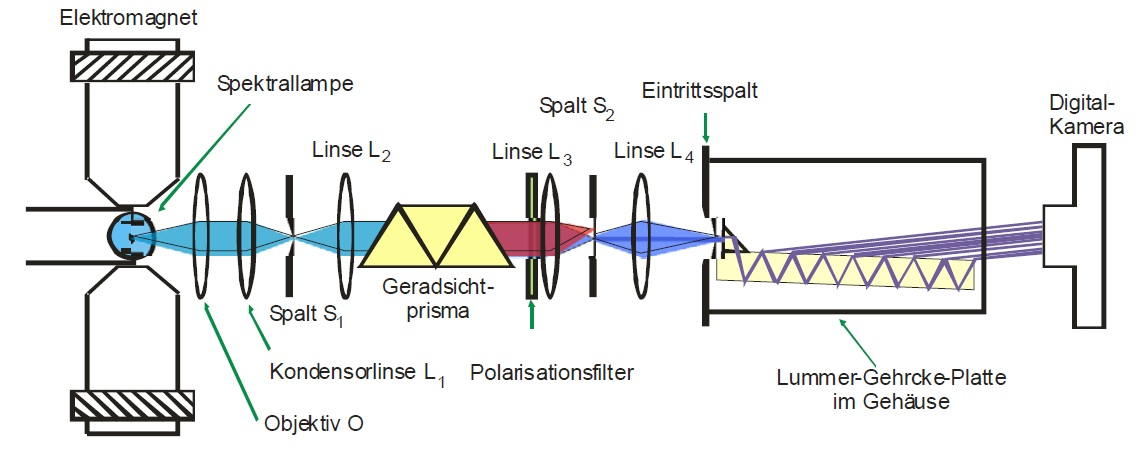
\includegraphics[width=0.9\linewidth]{Messapparatur.jpg}
		\caption{Messapparatur$^{[1]}$}
		\label{fig:messapparatur}
	\end{figure}
	Der Aufbau der Messapparatur ist in der Abbildung \ref{fig:messapparatur} schematisch dargestellt. Es wird eine Cadmium-Lampe zwischen den Elektromagneten gebracht. Das Licht wird senkrecht zur Magnetfeldrichtung kollimiert und auf ein Geradsichtprisma gelenkt, um die einzelnen Wellenlängen zu separieren, die dann auf den Spalt $S_2$ abgebildet werden. Dort kann ja dann die gewünschte Linie ausgewählt werden. Der vorgeschaltete Polarisationsfilter ermöglicht die Wahl der Polarisation. Zur Untersuchung des Zeeman-Effekts werden die roten und blauen Linien verwendet, die rote für den normalen Zeeman-Effekt und die blaue für den anormalen Zeeman-Effekt. Hinter dem Spalt S2 wird das Licht der Spektrallinie auf den Eintrittsspalt einer Lummer-Gehrcke-Platte gelenkt.
	Mit der Lummer-Gehrcke-Platte kann eine genaue Bestimmung der Wellenlänge des einstrahlenden Lichts mit Hilfe eines Interferenzverfahrens getroffen werden. Innerhalb der Platte wird das Licht mehrmals reflektiert, wobei jeder kleinen Teil des Lichts austreten kann. Werden diese Strahlen am Ende der Vorrichtung beobachtet, so kann dann konstruktive Interferenz genau auftreten, wenn die Bragg-Bedingung erfüllt ist:
	\begin{equation}
	2d\text{cos}(\theta) = n\lambda
	\end{equation}
	wobei $d$ die Dicke der Platte und $\lambda$ die Wellenlänge ist. Unter dem Einfluss eines Magnetfeldes verändert sich die Wellenlänge um $\delta\lambda$ und die Interferenzstreifen verschieben sich um $\delta s$.
	Das Dispersionsgebiet gibt die Differenz an, die zwei Wellenlängen maximal haben dürfen, um sich nicht zu überlagern:
	\begin{equation}
	\label{eq:dispersionsgebiet}
	\Delta \lambda_\text{D} = \frac{\lambda^2}{2d} \sqrt{\frac{1}{n^2-1}}.
	\end{equation}
	Das Auflösungsvermögen $A$ der Platte hängt von dem Brechungsindex $n$ und  der Wellenlänge $\lambda$ des verwendeten Lichtes:
	\begin{equation}
	\label{eq:auflösungsvermögen}
	A = \frac{\lambda}{\Delta\lambda} = \frac{L}{\lambda}(n^2-1).
	\end{equation}
	In diesem Versuch wird nun eine Hysteresekurve des benutzten Magnetfeldes aufgenommen($B$ in Abhängigkeit von $I$). Es werden mithilfe von einer Digitalkamera Bilder von der $\pi$-Linie und $\sigma$-Linie aufgenommen.
	
	\section{Vorbereitungsaufgabe}
	
	\subsection{Auflösungsvermögen und Dispersionsgebiet der Lummer-Gehrcke-Platte}
	Nach den Gleichungen \ref{eq:dispersionsgebiet} und \ref{eq:auflösungsvermögen} lassen sich nun das Dispersionsgebiet und das Auflösungsvermögen der Lummer-Gehrcke-Platte für die rote ($\lambda=\SI{643,8}{\nano\meter}$) und die blaue ($\lambda=\SI{480}{\nano\meter}$) Linie berechnen (siehe Tabelle \ref{tab:auflösungsunddispersion}). Die Berechnung erfolgt dabei mit $d=\SI{4}{\milli\meter}$, $L=\SI{120}{\milli\meter}$, $n($rot$)=1,4567$, $n($blau$)=1,4635$.
	
	\begin{table}[htpb]
		\centering
		\caption{Bestimmung des Auflösungsvermögens $A$ und des Dispersionsgebiets $\Delta\lambda_\text{D}$.}
		\label{tab:auflösungsunddispersion}
		
		\begin{tabular}{c| c| c}
			%\toprule 
			
			& $\lambda_\text{D} / \si{\pico\meter}$ & $A$ \\
			%\midrule
			\hline
			rot & 48,91 & 209129 \\
			blau & 27,0 & 285458 \\ 
			%\bottomrule
		\end{tabular}
	\end{table}
	
	\subsection{Termschemata der Spektrallinien}
	
	Die rote Linie entspricht einem Übergang $^1P_1\longleftrightarrow\,^1D_2$, die blaue $^3S_1\longleftrightarrow\,^3P_1$. Die Quantenzahlen und die nach Gleichung \eqref{eqn:lande} berechneten Landé-Faktoren der einzelnen Zustände sind aus der Tabelle \ref{tab:lande} zu entnehmen.
	Die Termschemata befindet sich in der Abbildung \ref{fig:termschemata}. 
	\begin{table}[h!]
		\centering
		\begin{tabular}{r|rrr|r}
			\hline\hline
			Zustand & $L$	&	$S$	&	$J$	&	$g_J$\\
			\hline\hline
			$^1P_1$ &	1	&	0	&	1	&	1\\
			$^1D_2$ &	2	&	0	&	2	&	1\\
			$^3S_1$ &	0	&	1	&	1	&	2\\
			$^3P_1$ &	1	&	1	&	1	&	$\frac{3}{2}$\\
			\hline
		\end{tabular}
		\caption{Die ausgerechneten Landé-Faktoren.}
		\label{tab:lande}
	\end{table}
	
	Für die Aufspaltung der Zeeman-Linien ergeben sich damit unter Beachtung von Gleichung \ref{eqn:Eanomal} die Energieunterschiede in Tabelle \ref{tabenergy}. Die Energiedifferenz ergibt sich dann zu:
	\begin{equation}
	\Delta E = g_{ij} \mu_\text{B} B
	\end{equation}
	wobei $g_{ij} = m_ig_i-m_jg_j$.
	\begin{table}[h]
		\begin{center}
			\begin{tabular}{c|ccc}
				&$\Delta m = -1$&$\Delta m = 0$&$\Delta m = +1$ \\ \hline
				rot & $\mu_{\text{B}} B$ & $0$ & $- \mu_{\text{B}} B$ \\
				blau ($m_1=+1$) & $\frac{3}{2} \mu_{\text{B}} B$ & $-\frac{1}{2} \mu_{\text{B}} B$ & - \\
				blau ($m_1=0$) & $2 \mu_{\text{B}} B$ & 0 & $-2 \mu_{\text{B}} B$ \\
				blau ($m_1=-1$) & - & $\frac{1}{2} \mu_{\text{B}} B$ & $-\frac{3}{2} \mu_{\text{B}} B$
			\end{tabular}
			\caption{Energieniveauunterschiede $\Delta E$ für ausgewählte Niveaus für $643{,}8\text{ nm}$ (rot) und $480 \text{ nm}$ (blau).}
			\label{tabenergy}
		\end{center}
	\end{table}
	
	\begin{figure}[H]
		\centering
		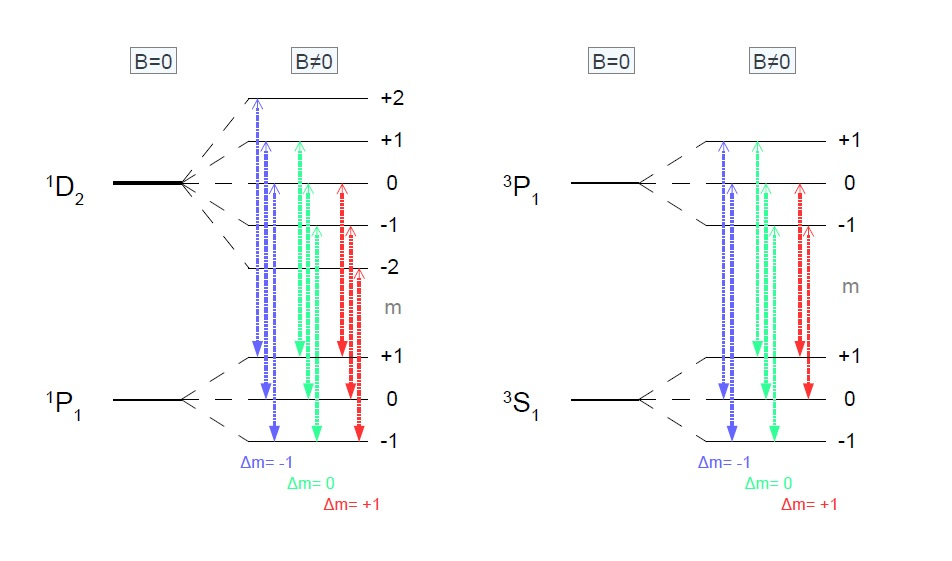
\includegraphics[width=0.9\linewidth]{Termschemata.jpg}
		\caption{Die Termschemata und die möglichen Übergänge$^{[2]}$}
		\label{fig:termschemata}
	\end{figure}
	

	
	
	
	
	\section{Auswertung}
	\subsection{Bestimmung des B-Feldes}
	In Tabelle 4 sind die eingestellten Stromstärken $I$ und die mit einer Hallsonde gemessene zugehörige Magnetfeldstärke $B$ aufgelistet. 
	
	\begin{table} [H]
		\centering
		\begin{tabular}{c|c} \hline
			Strom $I / A$ & Magn. Flussdichte $B / mT$ \\ 
			\hline 
			0 & 4 \\
			1 & 87 \\
			2 & 129 \\
			3 & 199 \\
			4 & 261 \\
			5 & 320 \\
			6 & 377 \\
			7 & 441 \\
			8 & 500 \\
			9 & 555\\
			10 & 611 \\
			11 & 673\\
			12 & 726 \\
			13 & 786 \\
			14 & 833 \\
			15 & 891 \\
			16 & 926 \\
			17 & 968 \\
			18 & 1003 \\
			19 & 1027 \\
			20 & 1057 \\
			\hline
		\end{tabular} 	
		
		\caption{Messwerte }
		\label {tab:threecols}
	\end{table}
Die Regressionskurve ist in Abbildung (7) gezeigt. 
\begin{figure}[H]
	\centering
	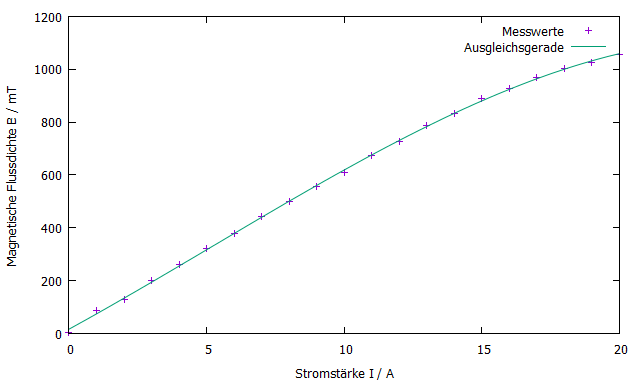
\includegraphics[height=8cm,width=12cm]{bfeld.png}
	\caption{ Das Magnetfeld in Abhängigkeit von der Stromstärke }
	\label{fig: abb. 1}
\end{figure} 

Die Ausgleichskurve hat die Form : 
\begin{align}
f(x)=ax^3+bx^2+cx+d
\end{align}
und die Berechnung der Parameter ergibt 
\begin{align*}
a=(-0,056 \pm 0,0081)\text{mT} \\
b=(0,869      \pm   0,2481) \text{mT}\\
c=( 57,192       \pm    2,105) \text{mT} \\
d= ( 16,225        \pm   4,743) \text{mT}
\end{align*}

\subsection{Bestimmung der Wellenlängenverschiebung }
\subsubsection{Rote Spektrallinie }
In Abbildung (8) sind für die Spektrallinie der Wellenlänge $\lambda$=643,8 nm aufgenommenen Interferenzbilder gezeigt. 

\begin{figure}[H]
	\centering
	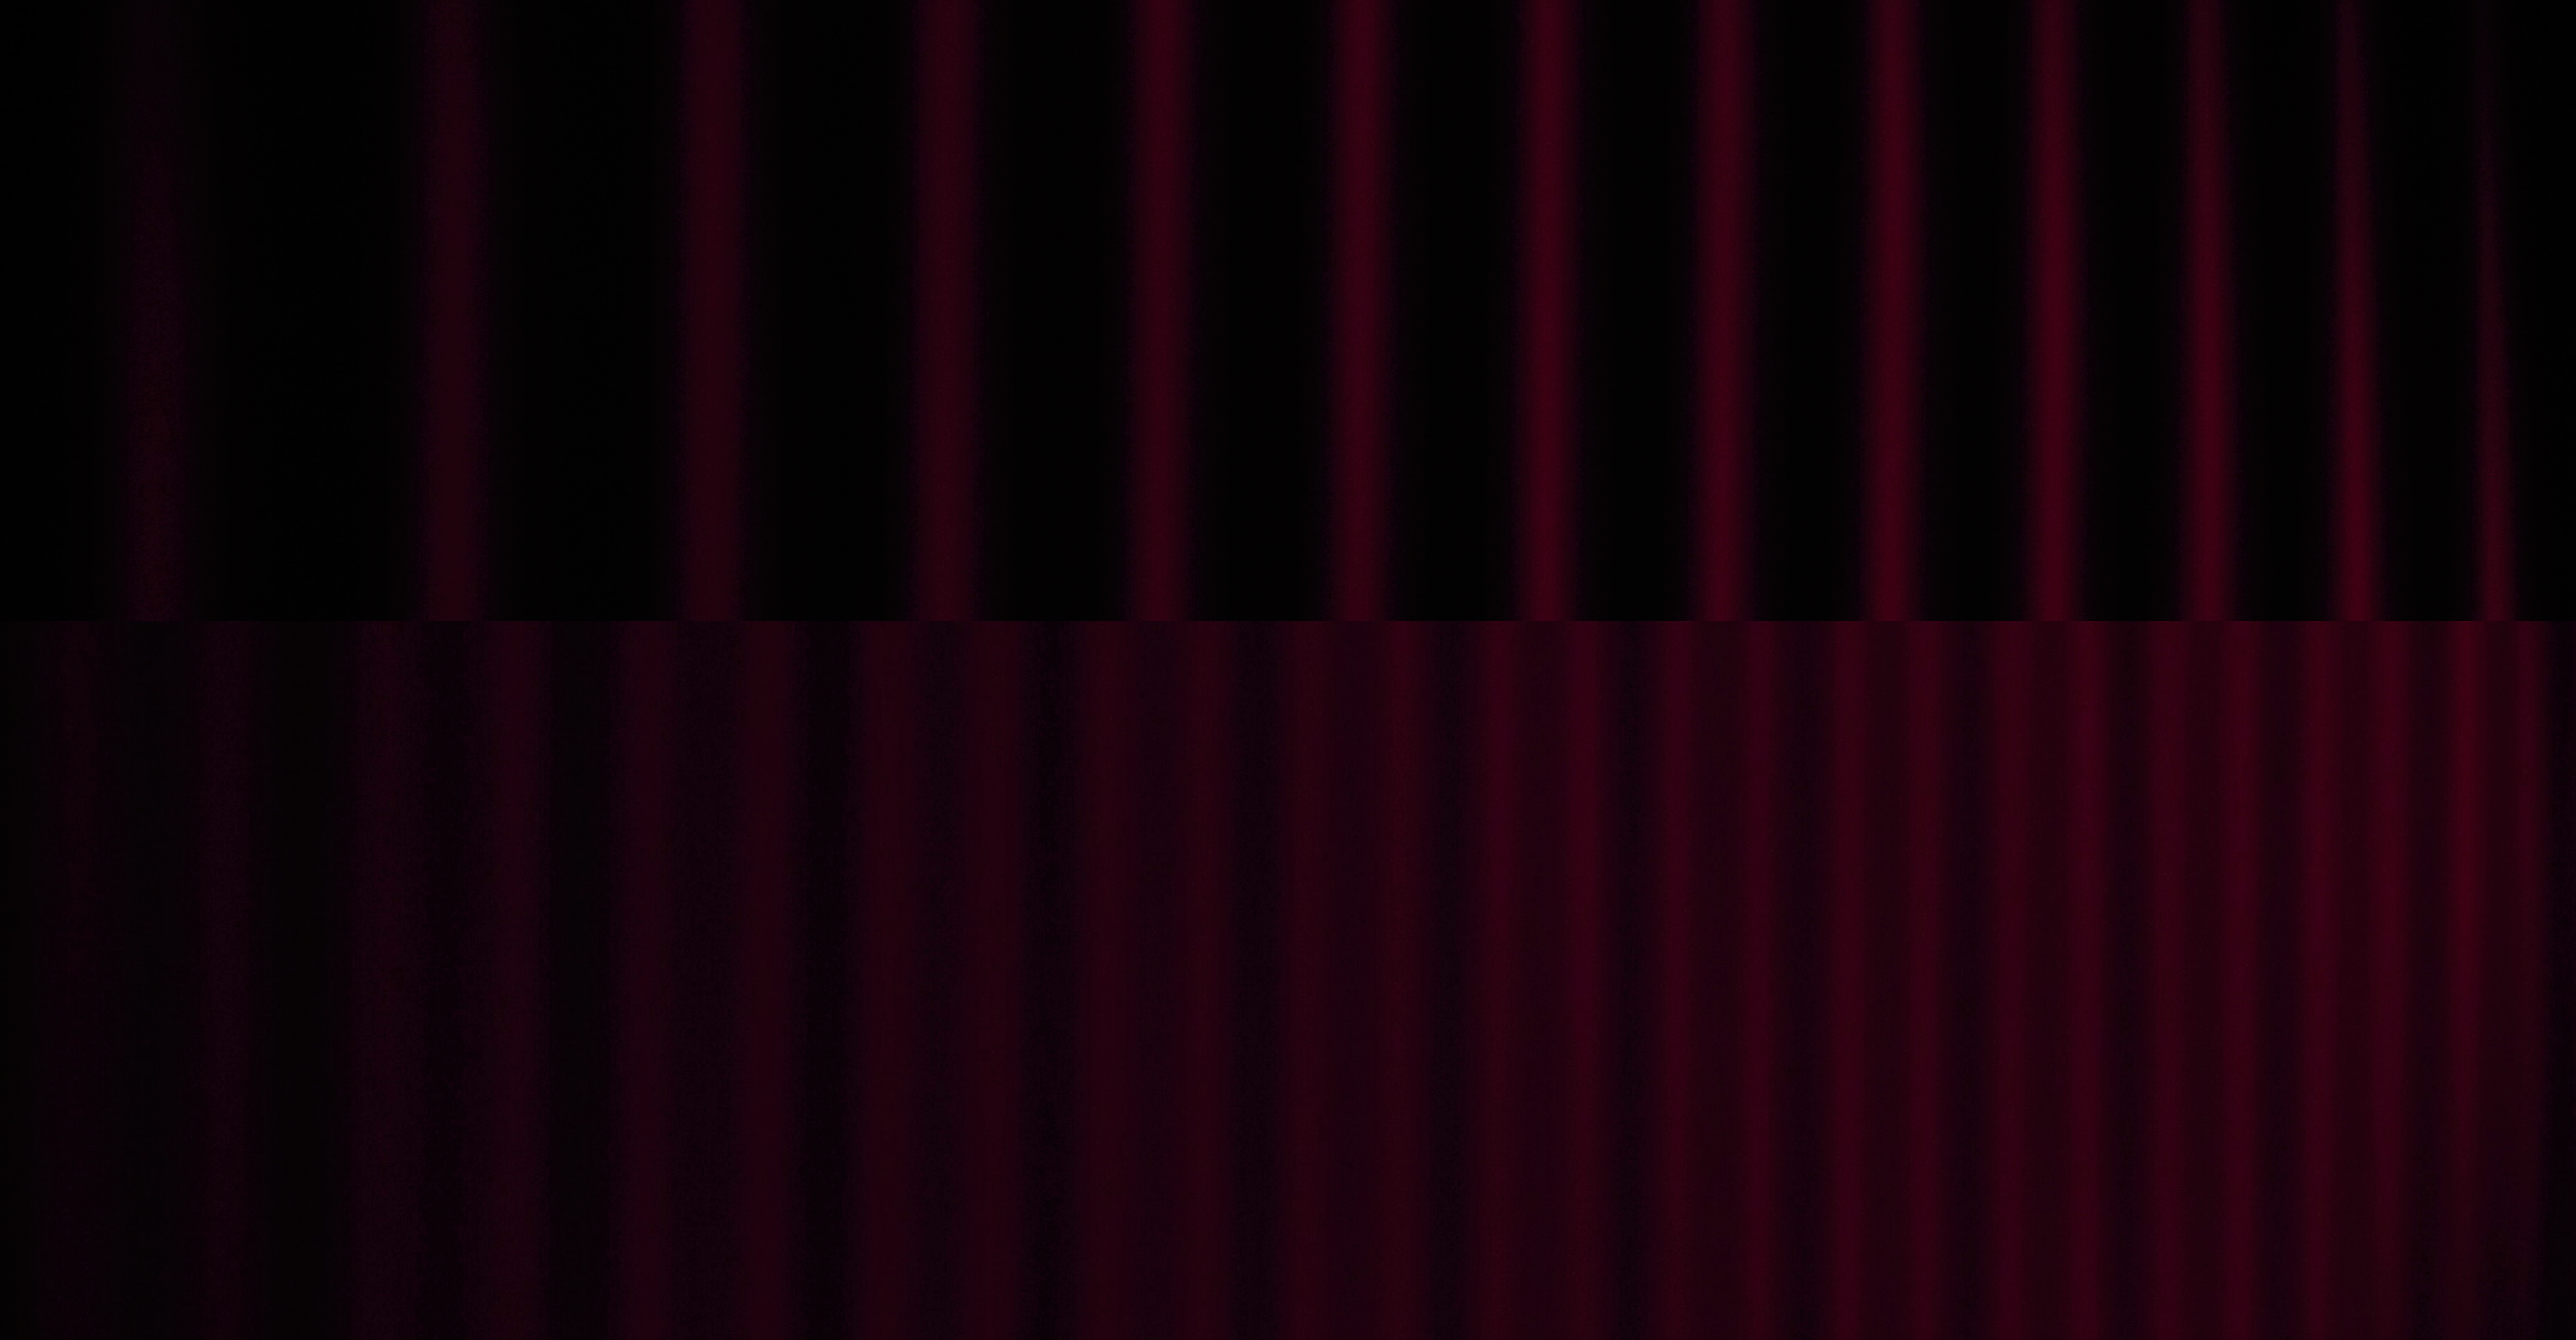
\includegraphics[height=7cm,width=11cm]{vergleichrotelinie.png}
	\caption{Interferenzmuster für das rote Licht, $\sigma$-Übergang }
	\label{fig: abb. 1}
\end{figure} 

Dabei entspricht das obere Muster dem Interferenzmuster bei ausgeschaltetem Magnetfeld (B=0) und das untere Muster dem Interferenzmuster bei eingeschaltetem Magnetfeld (B$\ne$0). Aus diesen Mustern wurden mittels Paint die in Tabelle aufgelisteten Werte ermittelt. Die Wellenlängenverschiebung wurde dabei mittels folgender Formel berechnet: 
\begin{align}
\delta\lambda= \dfrac{1}{2} \dfrac{\delta s}{\Delta s} \cdot \Delta \lambda_D
\end{align}
Es wird für jede Pixelanzahl $\Delta s$ und $\delta s$ eine Unsicherheit von $\pm$ 3 Pixeln angenommen, da per Augenmaß entschieden wird, wo die Maxima liegen. Damit besitzt jede einzelne Wellenlänge einen Fehler $F(\delta\lambda)$, der sich nach Gauß über 
\begin{align}
F(\delta \lambda)= \dfrac{1}{2}\Delta \lambda_D \sqrt{\left(\dfrac{1}{\Delta s}F(\delta s)\right)^2 + \left(\dfrac{\delta s}{\Delta s^2 }\cdot F(\Delta s)\right)^2}
\end{align}
berechnet. Dabei ist $F(\Delta s)=F(\delta s)=3$.

	
\begin{table} [H]
	\centering
		\caption{Abstände der Intensitätsmaxima und die daraus berechnete Wellenlängenverschiebung für $\lambda$=$\SI{643,8}{pm}$}
		\label {tab:threecols}
			\begin{tabular}{c|c|c|c} \hline		
		Ordnung & $\Delta s$ / $\#$ Pixel& $\delta s _{\sigma}$ / $\#$ Pixel& $\delta\lambda_{rot,\sigma}$ / pm \\ 
		\hline 
		1 & 320& 148& 6,23 $\pm$ 0,14 \\
		2 & 272 & 108& 5,35 $\pm$ 0,16 \\
		3 & 238 & 122 & 6,94 $\pm$ 0,19 \\
		4 & 224& 104& 6,25 $\pm$ 0,20 \\
		5 & 208& 96& 6,22 $\pm$ 0,21 \\
		6 & 188& 90& 6,4 5$\pm$ 0,24 \\
		7 & 186& 90& 6,52 $\pm$ 0,24\\
		8 & 176& 82& 6,28 $\pm$ 0,25 \\
		9 & 164& 68& 5,59 $\pm$ 0,27 \\
		10 & 158& 76& 6,48 $\pm$ 0,28\\
		11 & 154& 74& 6,48 $\pm$ 0,29 \\
		 
		
		\hline
	\end{tabular} 	
	
	\label {tab:threecols}
\end{table}
Die Mittelung über alle $\delta \lambda_i$ ergibt die Wellenlängenverschiebung 
\begin{align*}
\delta\lambda= (10,99\pm 0,11) \text{pm}.
\end{align*}
Der Fehler wurde mit Hilfe der Formel
\begin{align}
F(\delta \lambda)=\dfrac{1}{N}\sqrt{\sum_{i=1}^{N}F(\delta\lambda_i^2)}
\end{align}
bestimmt. 

\subsubsection{Blaue Linie}
Die Abbildung (9) zeigt das Interferenzmuster der Spektrallinien mit der Wellenlänge $\lambda$=450 nm für den $\pi$-Übergang. 

\begin{figure}[H]
	\centering
	
\includegraphics[height=7cm,width=11cm]{vergleichblaue1linie.jpg}
	\caption{ Ausschnitt des Interferenzmusters für die blaue Spektrallinie beim $\pi$-Übergang}
	\label{fig: abb. 1}
\end{figure} 

Im oberen Teil der Abbildung ist das Interferenzmuster bei ausgeschaltetem Magnetfeld (B=0) dargestellt. Im unteren Teil ist die Aufspaltung der Energieniveaus beim $\pi$-Übergang zu sehen (B$\ne$0). Auch hier werden die Maximaabstände bestimmt und in der Tabelle 6 aufgelistet. 
\begin{table} [H]
	\centering
	\caption{Abstände der Intensitätsmaxima und die daraus berechnete Wellenlängenverschiebung für $\lambda$=$\SI{480}{pm}$}
	\label {tab:threecols}
	\begin{tabular}{c|c|c|c} \hline		
		Ordnung & $\Delta s_{blau}$ / $\#$ Pixel& $\delta s_{blau,\pi}$ / $\#$ Pixel& $\delta\lambda_{blau,\pi}$ / pm \\ 
		\hline 
		1 & 447& 198& 5,97 $\pm$ 0,24 \\
		2 & 369 & 129& 4,71 $\pm$ 0,11 \\
		3 & 315 & 114 & 4,88 $\pm$ 0,14 \\
		4 & 276& 102& 4,98 $\pm$ 0,16 \\
		5 & 234& 93& 5,36 $\pm$ 0,19 \\
		6 & 222& 66& 4,01$\pm$ 0,19 \\
		7 & 204& 69& 4,56$\pm$ 0,21\\
		8 & 201& 63& 4,22 $\pm$ 0,21 \\
		9 & 180& 63& 4,72 $\pm$ 0,24 \\
		10 & 180& 66& 4,94 $\pm$ 0,24\\
		11 & 168& 63& 5,05 $\pm$ 0,26 \\
		
		
		\hline
	\end{tabular} 	
	
	\label {tab:threecols}
\end{table}
Die Mittelung ergibt eine Wellenverschiebung von 
\begin{align*}
\delta\lambda_{blau,\pi}=(4,85\pm0,06)\text{pm}
\end{align*}
und der Fehler wurde mit der Formel (27) bestimmt. \\\\
In der nächsten Abbildung 10 ist der $\sigma$-Übergang dargestellt. 
\begin{figure}[H]
	\centering
	
\includegraphics[height=7cm,width=11cm]{vergleichblaue2linie.jpg}
	\caption{ Ausschnitt des Interferenzmusters der blauen Spektrallinie beim $\sigma$-Übergang}
	\label{fig: abb. 1}
\end{figure} 

Im oberen Teil der Abbildung ist das Interferenzmuster bei ausgeschaltetem Magnetfeld zu sehen und im unteren Teil bei eingeschaltetem Magnetfeld. In der Tabelle sind die zugehörigen Maximaabstände bestimmt worden. 

\begin{table} [H]
	\centering
	\caption{Abstände der Intensitätsmaxima und die daraus berechnete Wellenlängenverschiebung für $\lambda$=$\SI{480}{pm}$}
	\label {tab:threecols}
	\begin{tabular}{c|c|c|c} \hline		
		Ordnung & $\Delta s_{blau}$ / $\#$ Pixel& $\delta s_{blau,\sigma}$ / $\#$ Pixel& $\delta\lambda_{blau,\sigma}$ / pm \\ 
		\hline 
		1 & 320& 148& 6,23 $\pm$ 0,14 \\
		2 & 272 & 108& 5,35 $\pm$ 0,16 \\
		3 & 238 & 122 & 6,91 $\pm$ 0,19 \\
		4 & 224& 104& 6,25 $\pm$ 0,20 \\
		5 & 208& 96& 6,22 $\pm$ 0,21 \\
		6 & 188& 90& 6,45$\pm$ 0,24 \\
		7 & 186& 90& 6,52$\pm$ 0,24\\
		8 & 176& 82& 6,28 $\pm$ 0,25 \\
		9 & 164& 68& 5,59 $\pm$ 0,27 \\
		10 & 158& 76& 6,48 $\pm$ 0,28\\
		11 & 154& 74& 6,48 $\pm$ 0,29 \\
		
		
		\hline
	\end{tabular} 	
	
	\label {tab:threecols}
\end{table}
Die Mittelung ergibt eine Wellenverschiebung von 
\begin{align*}
\delta\lambda_{blau, \sigma}=(6,25\pm0,07)\text{pm}.
\end{align*}
Der Fehler wurde mit der Formel (27) bestimmt. 

\subsection{Bestimmung der Landré-Faktoren}

Zur Berechnung der Landré-Faktoren wurde zunächst der Ansatz
\begin{align}
\Delta E= g \mu_BB
\end{align}
verwendet.
Umgestellt nach dem Landré-Faktor $g$ ergibt sich
\begin{align}
g=\dfrac{\Delta E}{\mu_B B}.
\end{align}
Dabei lässt sich $\Delta E$ bestimmen durch
\begin{align*}
\Delta E=E(\lambda + \delta \lambda)-E(\lambda)
\end{align*}
Durch Taylorentwicklung ergibt sich 
\begin{align}
\Delta E=\dfrac{\delta E}{\delta \lambda}\cdot E(\lambda)
\end{align}
Anschließend wird (31) mit $E(\lambda)=\dfrac{hc}{\lambda}$ in (30) eingesetzt und es folgt für den Landré-Faktor
\begin{align}
g=\delta\lambda\dfrac{hc}{\mu_B B\lambda^2}
\end{align}


Die Tabelle 8 zeigt die Berechnung der einzelnen Landré-Faktoren. Dazu wird die verwendete Stromstärke I benötigt mit der das zugehörige Magnetfeld mit Hilfe der Gleichung (25) bestimmt wird. 

\begin{table} [H]
	\centering
	\caption{ Berechnete Landré-Faktoren für die verschiedenen Übergänge}
	
	\label {tab:threecols}
	\begin{tabular}{c|c|c|c|c} \hline		
		$\lambda$ / nm & Übergang & I / A & B / mT &  g\\ 
		\hline 
	643,8& $\sigma$& 10&619,4 $\pm$ 16,45 &0,91 $\pm$ 0,03 \\
	480,0&$\pi$&20&1059,4 $\pm$ 21,56&0,43 $\pm$ 0,02\\
	480,0& $\sigma$&5&316,9$\pm$ 11,23&1,83 $\pm$ 0,05\\
		
		
		\hline
	\end{tabular} 	
	
	\label {tab:threecols}
\end{table}
Der Fehler F(B) berechnet sich nach der Gaußschen Fehlerfortpflanzung über 
\begin{align}
F(B)=\sqrt{(I^3\cdot \Delta a)^2+(I^2\cdot \Delta b)^2+(I\cdot\Delta c)^2+(\Delta d)^2}
\end{align}
und der Fehler F(g) auf den Landré-Faktor mit
\begin{align*}
F(g)= \dfrac{hc}{\lambda^2 \mu_B}\sqrt{\left(\dfrac{1}{B}\cdot F(\delta\lambda)\right)^2+\left(\dfrac{\delta\lambda}{B^2}\cdot F(B)\right)^2}
\end{align*}

\section{Diskussion}
In der Tabelle 9 sind die experimentell ermittelten und die theoretischen Landré-Faktoren und deren prozentuale Abweichung aufgetragen. 

\begin{table} [H]
	\centering
	\caption{Theoretisch und aus den Interferenzbildern berechnete Landré-Faktoren g}
	\label {tab:threecols}
	\begin{tabular}{c|c|c|c|c} \hline		
		$\lambda$ / nm & Übergang & $g_{theo}$ & $g_{exp}$ &  Abweichung / $\%$\\ 
		\hline 
		643,8& $\sigma$& 1.0 &0,91 $\pm$ 0,03 &9\\
		480,0&$\pi$&0,5&0,43 $\pm$ 0,02& 14\\
		480,0& $\sigma$&1,75&1,83 $\pm$ 0,05&4\\
		
		
		\hline
	\end{tabular} 	
	
	\label {tab:threecols}
\end{table}

Alle drei experimentell ermittelten Landré-Faktoren weisen eine Abweichung zu den Theoriewerten auf. Die größte Abweichung beträgt 14$\%$ beim $\pi$-Übergang im blauen Wellenlängenbereich. Bei den $\sigma$-Übergängen liegen sowohl für den roten als auch für den blauen Wellenlängenbereich die Abweichungen in einem akzeptablen Bereich. Für den $\sigma$-Übergang des blauen Lichtes gibt es zwei Landré-Faktoren $g_1=1,5$ und $g_2=2$. Aufgrund des Doppler-Effektes und des zu kleinen Dispersionsgebietes verbreiten und überlappen sich die Linien, sodass die Energieaufspaltung nicht zu erkennen ist. Somit wird für den $\sigma$-Übergang der Mittelwert $g=1,75$ genommen. Allgemein unterlag der Versuch mehreren Fehlerquellen, die die oberen Abweichung in der Tabelle verursachen könnten. Zunächst ist zu erwähnen, dass die mit der Digitalkamera aufgenommenen Bilder teilweise dunkel und unscharf waren, sodass es nötig war diese Bilder im Computer zu bearbeiten. Auch die Eingrenzung der einzelnen Maximaabstände wurde per Augenmaß bestimmt. Zudem konnte das Magnetfeld nicht exakt an der Stelle, an der sich die Cd-Lampe befand, ausgemessen werden. Es ist davon auszugehen, dass der gemessene Wert des Magnetfeldes vom realen Wert abweicht und es so zu Abweichungen in der Rechnung führte. Auch das Ablesen der Stromstärke an der Anzeige unterlag gewissen Schwankungen, sodass es zu weiteren Messfehlern führte. 
\section{Literatur}
[1] TU Dortmund, Anleitung zum Versuch 27: Zeeman-Effekt\\
http://129.217.224.2/HOMEPAGE/PHYSIKER/BACHELOR/FP/SKRIPT/V27.pdf (besucht am 10.11.2018)\\\\
$[2]$ Lars Klompmaker und Fabian Lehmann. Versuch 27: Zeeman-Effekt, Abbildung 9: Die Termschemata der betrachteten Linien, S.5.2018
\end{document}